\section{Durchführung}

\subsection{Versuchsaufbau}
Ein Schaltplan des Versuchsaufbaus ist in Abbildung \ref{fig:schaltung} zu sehen.
\begin{figure}[H]
    \centering
    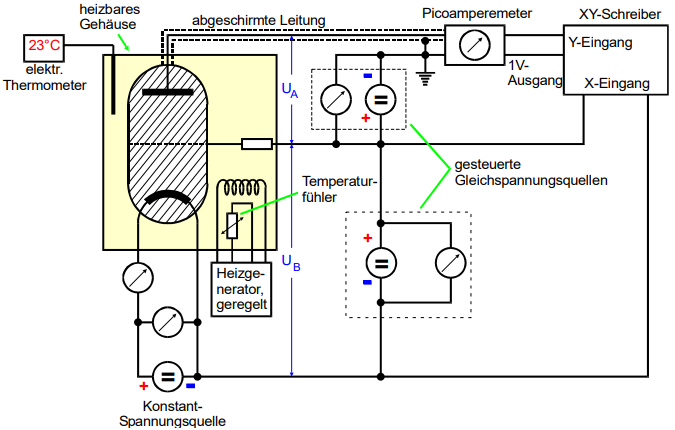
\includegraphics[height = 7.5cm]{bilder/schaltung.png}
    \caption{Schaltplan des Versuches \cite{man:v601}.}
    \label{fig:schaltung}
\end{figure}

\noindent
Das Glasrohr mitsamt der Elektroden, dem Glühdraht und dem Hg-Dampf befinden sich in einem heizbaren Gehäuse.
Die Innentemperatur $T$ kann mittels eines elektronischen Temperaturreglers eingestellt werden.
%wobei hier allerdings Schwankungen auftreten.
Die Temperatur selbst kann an einem elektronischen Thermometer abgelesen werden.
Der Glühdraht ist an eine Konstantspannungsquelle angeschlossen.
Die Beschleunigungselektrode ist an eine Gleichspannungsquelle angeschlossen, deren Variationsbereich zwischen 0 und $\qty{60}{\volt}$ liegt.
Die Spannungsquelle der Auffängerelektrode hat einen Bereich von 0 bis $\qty{11}{\volt}$.
Mit Hilfe eine Picoamperemeters kann der Auffängerstrom $I_\text{A}$ gemessen werden.
Der Strom $I_\text{A}$ kann mit Hilfe eines xy-Schreibers je nach Messreihe in Abhängigkeit von $U_\text{A}$ bzw. $U_\text{B}$ aufgezeichnet werden.

\subsubsection{Einstellen der Temperatur}
Das Einstellen des erforderlichen Dampfdurckes $p_\text{sät}$ erfolgt über die Temperatur $T$, vgl. Abschnitt \ref{sec:dampfdruck}.
Zum Erhitzen des Gehäuses wird der entsprechende Stellknopf am Temperaturregler nach rechts gedreht. 
Der Ausgangsstrom des Reglers steigt beim Erhitzen auf einen Wert von ca. $\qtyrange[]{2.1}{2.2}{\ampere}$.
Sobald das Thermometer die Tempereatur anzeigt, die gewünscht ist, wird der Regler so weit zurück gedreht, bis eine Stromstärke von ca. $\qty[]{1.2}{\ampere}$ angezeigt wird.
Wenn der Strom anschließend zwischen den genannten Werten pendelt, wird die Temperatur idealerweise konstant gehalten.
Es sei angemerkt, dass $T$ auch nach dem Einstellen Schwankungen von $\pm \qty[]{10}{\celsius}$ hat und dementsprechend ungenau ist.

\subsubsection{Der xy-Schreiber}
Die jeweilige Spannung wird am x-Eingang und der Strom am y-Eingang angelegt.
Die Spannung, die der y-Eingang eigentlich benötigt, kommt dabei aus dem Picoamperemeter.
Zum Zeichnen wird (Millimeter-)Papier elektrostatisch auf der Oberfläche des Schreibers fixiert. 
Der Schreiber wird eingestellt, indem zunächst mit den Knöpfen \enquote{zero} die Nullpunkte der beiden Eingänge festgelegt werden.
Dabei darf kein Signal auf den Eingängen liegen.
Anschließend wird die maximale Auslenkung in x-Richtung dem jeweiligen Spannungsmaximum der Spannungsquellen angepasst.
Es werden einige Zwischenwerte für die Spannung markiert.
Auf der y-Achse soll ein Wert von ca. $I_\text{A} = \qty[]{3}{\nano\meter}$ noch etwas unterhalb des Vollausschlages liegen. 
Auch hier werden Zwischenwerte notiert.


\subsection{Integrable Energieverteilung der Elektronen}
\label{sec:enegieverteilung}
Zum Messen der integrablen Energieverteilung der Elektronen wird eine konstante Beschleunigungsspannung $U_\text{B} = \qty[]{10}{\volt}$ eingestellt.
Am x-Eingang des xy-Schreibers wird die Bremsspannung $U_\text{A}$ angelegt.
Es findet jeweils eine Messung bei annähernder Zimmertemperatur $T = \qty[]{24.4}{\celsius}$ (Messung A) und bei ca. $T = \qty[]{145}{\celsius}$ (Messung B) statt.
In der ersten Messung wird $I_\text{A,1} = \qty[]{2.55}{\nano\ampere}$ als y-Achsenabschnitt eingestellt, in der zweiten $I_\text{A,2} = \qty[]{2.05}{\nano\ampere}$.
Das vorgehen ist in beiden Teilen gleich: 
Nach dem Justieren des Schreibers bzw. der Empfindlichkeit und ggf. Einstellen von $T$ wird der Deckel des Stiftes am Schreiber entfernt 
und der Stift auf das Papier gebracht.
Ausgehend von $\qty[]{0}{\volt}$ wird die Spannung $U_\text{A}$ mit Hilfe der Schalter \enquote{Start/Stopp} und \enquote{steigend/fallend} 
am Spannungsgerät kontinuierlich erhöht.
Sobald die maximale Spannung erreicht ist, wird der Deckel auf den Stift gesetzt und das Papier aus dem Schreiber genommen.
Danach werden die nötigen Werte/ Größen werden auf dem Papier notiert.

\subsection{Franck-Hertz-Kurven}
Zum Messen der Franck-Hertz-Kurven wird eine konstante Bremsspannung $U_\text{A} = \qty[]{1}{\volt}$ angelegt.
Am x-Eingang des Schreibers wird nun die Beschleunigungsspannung $U_\text{B}$ angelegt.
Bei der ersten Messung (C) schwankt die eingestellte Temperatur ca. zwischen $\qtyrange[]{157}{170}{\celsius}$,
beim zweiten Teil (D) ca. zwischen $\qtyrange[]{185}{197}{\celsius}$.
Der restliche Ablauf erfolgt in beiden Teilen analog zu Abschnitt \ref{sec:enegieverteilung}.